\chapter{Mejoras visuales}
				
En el capítulo anterior se definió la implementación básica para visualizar una escena simple. Así pues, este capítulo explica las mejoras visuales más comunes utilizadas en los motores gráficos de producción, así como su implementación en Eleven Renderer y su evaluación.
	
\section{Desenfoque: Modelo de lente fina}
	
Hasta ahora se ha estado utilizando un modelo de cámara ideal denominado cámara estenopeica. Esta cámara tiene la particularidad de tener un enfoque perfecto siempre, siendo una propiedad indeseada en un motor de renderizado fotorrealista, esto se debe a que a diferencia de las cámaras estenopeicas, , las cámaras reales incluyen lentes en su estructura que desvían los rayos de luz gracias a la difracción del cristal, enfocando a determinada distancia, y desenfocando el resto de la escena. El hecho de poder enfocar a una distancia determinada permite hacer énfasis en un sujeto de la escena y desenfocar el resto. Este efecto se conoce como \emph{Bokeh} y es muy deseado en un motor de renderizado, puesto que es un recurso cinematográfico muy atractivo visualmente.

Para solventar el problema del enfoque perfecto se hace uso de un modelo de cámara denominado modelo de lente fina. Este modelo es una simplificación de lo que sería una simulación física de unas lentes reales. Al simplificar los cálculos, se pierden artefactos y desperfectos deseados como la aberración cromática o la distorsión de lentes, pero a cambio se obtiene la simplicidad de implementación.

Para activar este efecto, es necesario compilar con la constante \code{BOKEH} definida. Esto desbloqueará la parte del código que hace el cálculo del desenfoque, ubicado en \autoref{cod:bokeh} 
	
Este nuevo método añade a la clase \code{Camera} dos nuevas variables, por un lado \code{focusDistance} y por otro lado \code{aperture}. La primera define la distancia a la que se encuentra el plano de enfoque, y la segunda, la apertura en f-stops del iris de la cámara. 

El procedimiento para calcular los rayos emitidos por el nuevo modelo de cámara se muestra de manera visual en la \autoref{cod:bokeh} y es el siguiente:

\begin{enumerate}
		
\item Se calcula el rayo original del método anterior, desde la cámara hasta el sensor.

\item Se calcula la intersección de dicho rayo con el plano de enfoque, situado a la distancia \code{focusDistance}. La intersección se denomina \code{focusPoint}.
	
\item En vez de emitir el rayo desde el punto de la cámara, se elige un punto aleatorio en el iris \code{iRP} y se emite un rayo desde ahí hasta el punto de enfoque \code{focusPoint}. Este nuevo rayo será un rayo bajo el modelo de cámara de lente fina. Los elementos situados a la distancia de enfoque \code{focusDistance} serán más nítidos que aquellos que no lo estén.
	
\end{enumerate}

\begin{minipage}[c]{0.95\textwidth}
\begin{lstlisting}[label={cod:bokeh}, caption={Código de desenfoque.}]
	
	#if BOKEH
	
    float rIPx, rIPy;

    // The diameter of the camera iris
    float diameter = camera.focalLength / camera.aperture;

    // Total length from the camera to the focus plane
    float l = camera.focusDistance + camera.focalLength;

    // The point from the initial ray which is actually in focus
    Vector3 focusPoint = ray.origin + ray.direction * l;

    // Sampling for the iris of the camera
    uniformCircleSampling(r3, r4, r5, rIPx, rIPy);

    rIPx *= diameter * 0.5;
    rIPy *= diameter * 0.5;

    Vector3 orig = camera.position + Vector3(rIPx, rIPy, 0);

    //Blurred ray
    ray = Ray(orig , focusPoint - orig);

	#endif 

\end{lstlisting}
\end{minipage}

\begin{figure}[H]
	\centering
	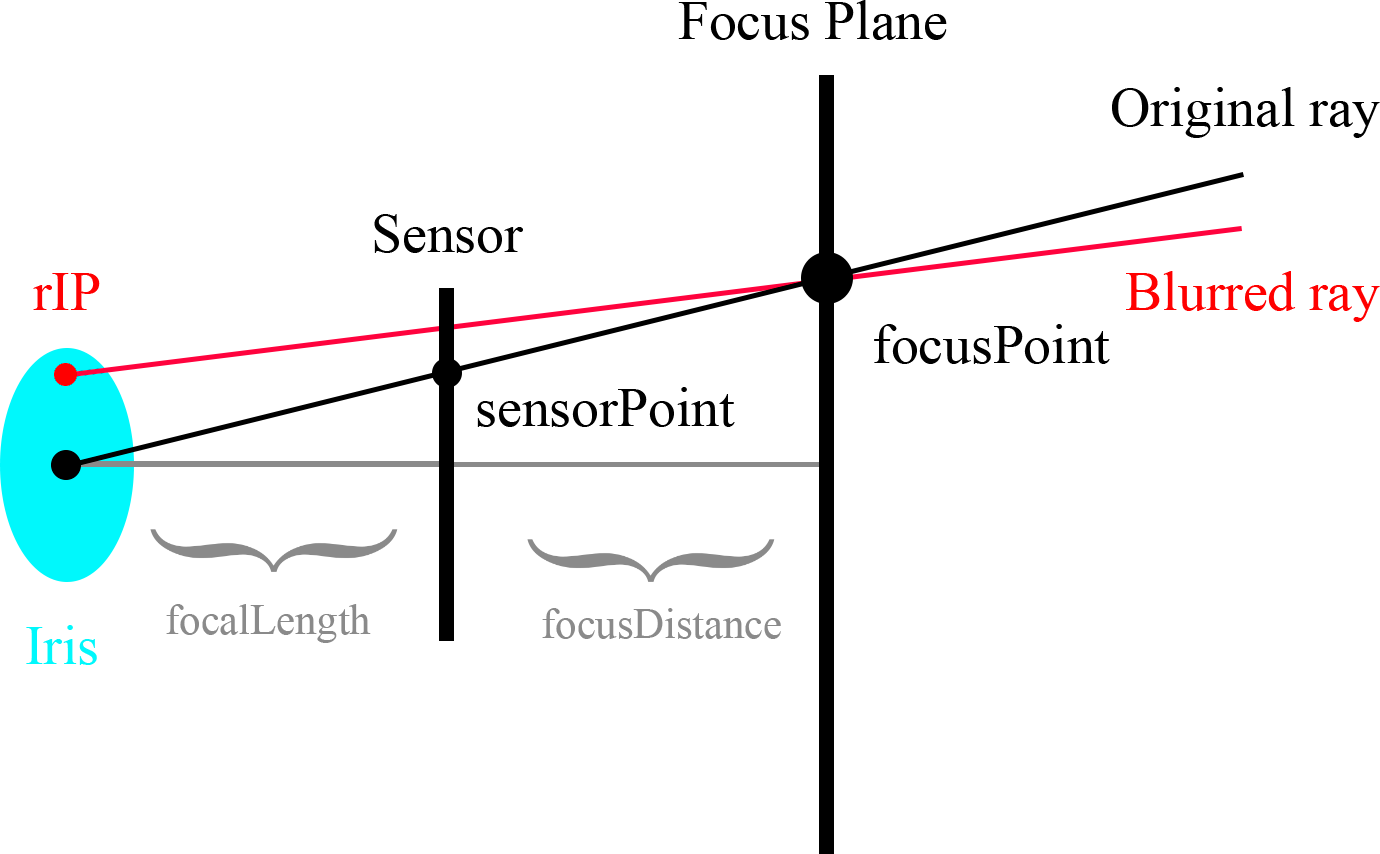
\includegraphics[width=0.7\textwidth]{blurring}
	\caption{Esquema cámara modelo de lente fina.}
	\label{fig:thinlensecamera}
\end{figure}

El resultado final es un desenfoque configurable a partir de la distancia de enfoque. Es posible, también, aumentar la cantidad de desenfoque reduciendo el número de f-stops, que consecuentemente aumentará la apertura del iris. La \autoref{fig:focusboxes} muestra un ejemplo de la modificación de distancia de enfoque mencionada.

\begin{figure}[H]
	\centering
  \begin{minipage}[b]{0.3\textwidth}
	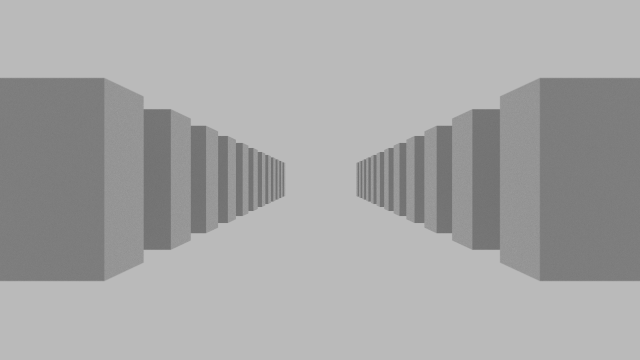
\includegraphics[width=\textwidth]{nofocus}
	\caption{Desenfoque desactivado.}
  \end{minipage}
  \hfill
  \begin{minipage}[b]{0.3\textwidth}
	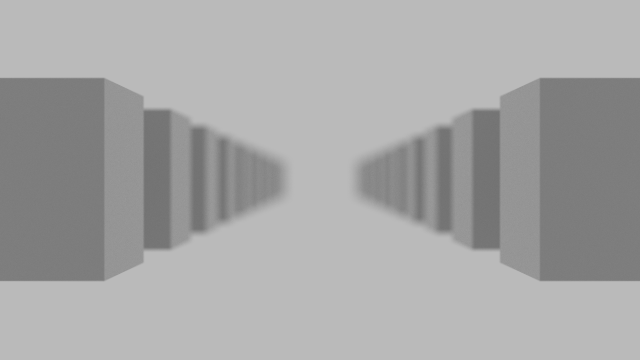
\includegraphics[width=\textwidth]{focusnear}
	\caption{Distancia de enfoque 10m.}
  \end{minipage}
  	\hfill
  \begin{minipage}[b]{0.3\textwidth}
	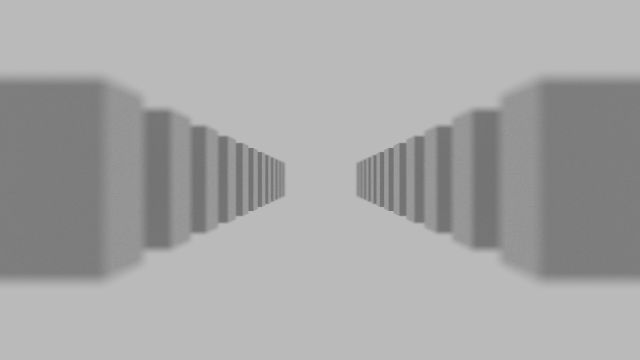
\includegraphics[width=\textwidth]{focusfar}
	\caption{Distancia de enfoque 30m.}
  \end{minipage}
\caption{Comparación de distintas distancias de enfoque.}
\label{fig:focusboxes}
\end{figure}
	
		
\section{Texturas}
	
El uso de colores planos en los materiales limita la capacidad de imitación de la realidad. Un recurso esencial para romper esta limitación es el uso de texturas. Una textura consiste en una matriz bidimensional de valores en punto flotante. En la implementación se ha añadido una clase \code{Texture} que contiene dos valores enteros \code{width} y \code{height}, que indican la altura y anchura de la matriz de datos \code{data}. La carga se hace a partir de un constructor que toma como parámetro la dirección de una imagen en formato .bmp y dividirá el valor de cada canal y cada pixel por 256 con el fin de limitar el rango de valores en [0,1). Los valores \code{width} y \code{height} son extraídos de la cabecera. El constructor admite un parámetro opcional \code{colorSpace}, que determina si es necesario convertir la imagen cargada de espacio de color. Por el momento, solo se soportan dos espacios de color, el espacio Lineal y el espacio sRGB, que son los más comunes.

Para cambiar de Lineal a sRGB se eleva el valor a 2.2, que es el valor de corrección de gamma. Para cambiar de sRGB a Lineal, se eleva el valor a $\frac{1}{2.2}$.
	
	%@todo add image of a color texture
	
\subsection{Mapeo}

Puesto que cada textura puede tener distintas resoluciones, es bastante útil definir un sistema de coordenadas relativas a la altura y anchura de una textura. Este sistema se conoce como sistema de coordenadas \code{u,v}. Ambas coordenadas \code{u} y \code{v} son valores de punto flotante comprendidos entre [0,1]. \code{u} indica la coordenada horizontal mientras que \code{v} indica la coordenada vertical. Estas coordenadas son diferentes a las coordenadas \code{u,v} explicadas en \hyperref[subsec:triintersection]{Intersección triángulo - rayo} aunque tengan el mismo nombre.

También resulta útil definir dos parámetros de transformación para las texturas. Estos son \code{Tile} y \code{Offset}. El primero indica el inverso de la escala de la textura; útil, por ejemplo, si se busca que una textura se repita cierto número de veces. El segundo es el desplazamientos de esta en dos ejes. Dicha transformación queda contemplada en \autoref{cod:getval}

\begin{minipage}[c]{0.95\textwidth}
\begin{lstlisting}[label={cod:getval}, caption={Código para obtener valor de una textura.}]
	
	__host__ __device__ Vector3 getValueFromCoordinates(int x, int y) {
	
        Vector3 pixel;

        // Offset and tiling tranforms
        x = (int)(xTile * (x + xOffset)) % width;
        y = (int)(yTile * (y + yOffset)) % height;

        pixel.x = data[(3 * (y * width + x) + 0)];
        pixel.y = data[(3 * (y * width + x) + 1)];
        pixel.z = data[(3 * (y * width + x) + 2)];

        return pixel;
    }
\end{lstlisting}
\end{minipage}

\subsection{IBL (Image Based Lightning)}
	
Hasta ahora, la luz que llegaba a la escena desde el fondo era una radiación homogénea determinada por un color, sin embargo, es posible utilizar imágenes para iluminar la escena.
	
La iluminación basada en imagen ha sido uno de los elementos más relevantes en las técnicas para el renderizado fotorrealista. Se utiliza ampliamente en la industria cinematográfica debido a la complejidad visual que aporta a una escena 3D porque permite captar la iluminación de entornos reales y posteriormente añadirla en escenas digitales. El hecho de poder trasladar la iluminación a un escenario virtual facilita la composición de modelos tridimensionales en películas y series de televisión, donde es necesario juntar una grabación real con un elemento generado por ordenador.

Esta técnica se basa principalmente en usar una fotografía de 360 grados como fuentes de luz formando una esfera alrededor de la escena. Estas fotografías son conocidas como HDRI (del inglés High Dynamic Range Image). A diferencia de las imágenes tradicionales, las cuales normalmente tienen 8 bits de resolución por canal de color, las imágenes HDRI cuentan con valores de punto flotante. El uso de las imágenes HDRI no se limita a la visualización de estas en pantallas de 8 bits de resolución por color como la mayoría de imágenes, sino que el valor de cada píxel será utilizado para realizar las operaciones pertinentes para iluminar la escena. Un ejemplo de este tipo de iluminación se aprecia en la \autoref{fig:hdriexample}

		
\begin{figure}[H]
	\label{fig:hdriexample}
    \centering
	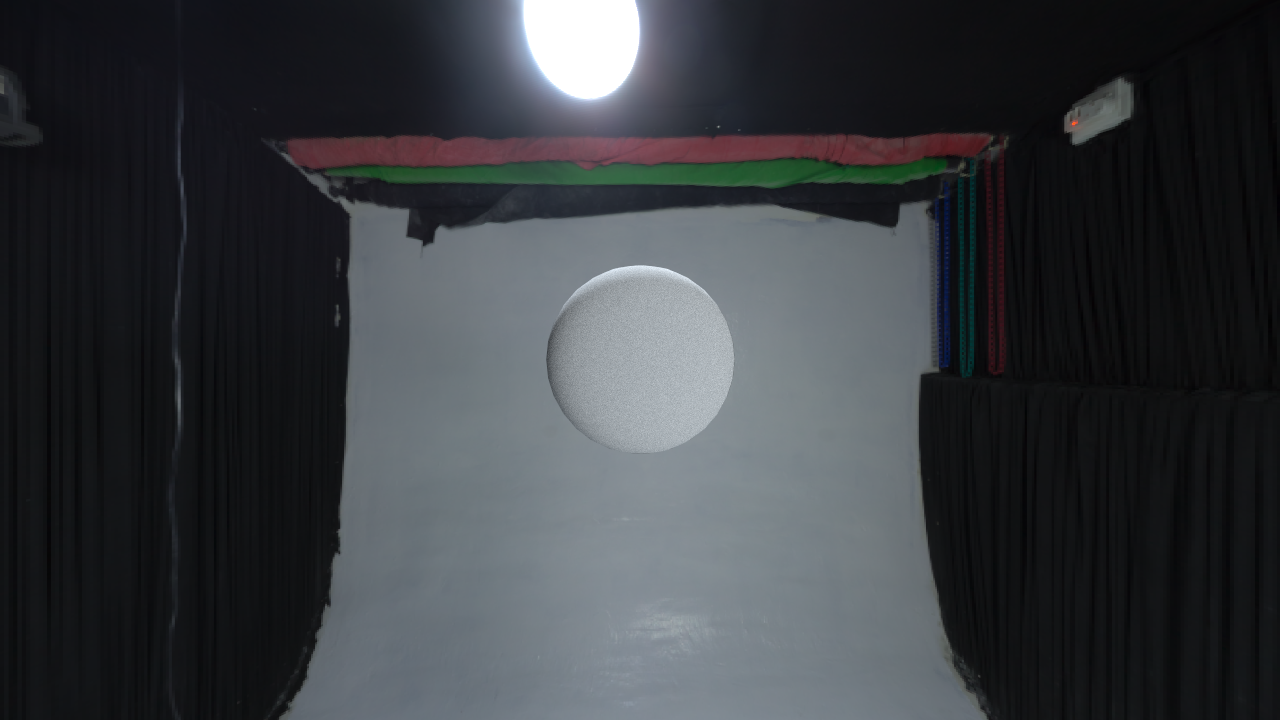
\includegraphics[width=0.7\textwidth]{hdriexample}
	\caption{Escena iluminada con una imagen HDRI de estudio, nótese como la luz superior incide directamente en la esfera acorde a la dirección.}
\end{figure}

La implementación de esta técnica en el motor de render viene dada por el uso de una imagen en formato .hdr (imágenes en punto flotante). Cada píxel de esta imagen se interpreta como una pequeña fuente de luz direccional en el infinito, orientada hacia el centro de la escena. Así pues, los rayos que no interseccionan en la escena con ningún elemento se considera que interseccionan en el infinito con el \code{HDRI}. Por esta razón, al detectar que un rayo sale de la escena, se obtiene su dirección, y esta dirección se traduce en las coordenadas polares de la imagen \code{HDRI}. Una vez se tienen las coordenadas polares, es posible obtener el valor lumínico del píxel al que apunta dicho rayo. Este será el valor lumínico que se utilice para dicho camino.
	

Debido a la naturaleza esférica de los mapas de entorno, resulta útil añadir dos funciones que transforman coordenadas esféricas en coordenadas \code{u,v}. Estas dos funciones son \code{sphericalMapping}, definida en \autoref{cod:sphericalmapping} y su inversa \code{reverseSphericalMapping}, definida en \autoref{cod:reversesphericalmapping}. La primera devuelve las coordenadas \code{u,v} para un punto situado en la superficie de una esfera de radio arbitrario mientras que la segunda calcula la posición de un punto en la superficie de una esfera de radio unitario, dadas dos coordenadas \code{u,v}.

\label{sphericalmapping}

\begin{minipage}[c]{0.95\textwidth}
\begin{lstlisting}[label={cod:sphericalmapping}, caption={Código para calcular las coordenadas u,v a través de un vector en una esfera de radio determinado.}]
	
    __host__ __device__ static inline void sphericalMapping(Vector3 origin, Vector3 point, float radius, float& u, float& v) {

        // Point is normalized to radius 1 sphere
        Vector3 p = (point - origin) / radius;

        float theta = acos(-p.y);
        float phi = atan2(-p.z, p.x) + PI;

        u = phi / (2 * PI);
        v = theta / PI;

        limitUV(u,v);
    }
	
\end{lstlisting}
\end{minipage}

\begin{minipage}[c]{0.95\textwidth}
\begin{lstlisting}[label={cod:reversesphericalmapping}, caption={Función inversa al mapeo esférico.}]
		
	__host__ __device__ static inline Vector3 reverseSphericalMapping(float u, float v) {

        float phi = u * 2 * PI;
        float theta = v * PI;

        float px = cos(phi - PI);
        float py = -cos(theta);
        float pz = -sin(phi - PI);

        float a = sqrt(1 - py * py);

        return Vector3(a * px, py, a * pz);
    }
	
\end{lstlisting}
\end{minipage}


\subsection{Filtrado}
			
Las texturas cuentan con valores discretos y resoluciones limitadas. Esto provoca que la imagen se pixele cuando se muestra cercana a la cámara. Una solución adoptada de manera general en muchos ámbitos es la interpolación de los píxeles vecinos. Actualmente, muchos visualizadores de imágenes no muestran los píxeles naturales, sino una versión modificada de estos. Esto se conoce como filtrado. En la implementación se ha usado un filtrado lineal conocido como interpolación bilineal. Este tipo de filtrado es sencillo de entender e implementar. El valor del punto \code{x} comprendido entre los cuatro píxeles más cercanos \code{v1-v4} es la suma ponderada de la distancia del punto a cada píxel en cada dimensión.
	
\begin{figure}[H]
	\label{fig:bilinear}
	\centering
	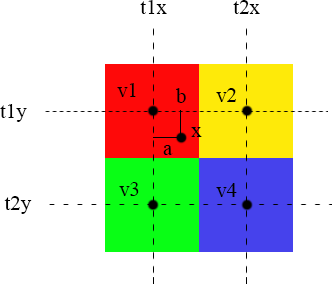
\includegraphics[width=0.3\textwidth]{bilinear}
	\caption{Interpolación bilineal.}
\end{figure}
	
\begin{minipage}[c]{0.95\textwidth}
\begin{lstlisting}[label={cod:bilinear}, caption={Código interpolación bilineal.}]
	
	__host__ __device__ Vector3 getValueBilinear(float u, float v) {
        
        float x = u * width;
        float y = v * height;

        float t1x = floor(x);
        float t1y = floor(y);

        float t2x = t1x + 1;
        float t2y = t1y + 1;

		// Weights per dimension
        float a = (x - t1x) / (t2x - t1x);
        float b = (y - t1y) / (t2y - t1y);

		// Rounded neighbour values
        Vector3 v1 = getValueFromCoordinates(t1x, t1y);
        Vector3 v2 = getValueFromCoordinates(t2x, t1y);
        Vector3 v3 = getValueFromCoordinates(t1x, t2y);
        Vector3 v4 = getValueFromCoordinates(t2x, t2y);

		// Linear interpolation
        return lerp(lerp(v1, v2, a), lerp(v3, v4, a), b);
	}
\end{lstlisting}
\end{minipage}	

Este método introduce cuatro lecturas del valor de la textura en vez de la única lectura sin usar técnicas de filtrado, de manera que resulta conveniente analizar el posible impacto en la eficiencia. Para comprobar esto se ha renderizado la misma escena con y sin filtrado en la \autoref{fig:filtercomparaison}. 
	
El render sin filtrado es un 0.8\% más rápido, una penalización poco sustancial, por lo que se utilizará el filtrado bilinear de manera predeterminada. Se esperaría que esta penalización fuera mayor debido a la multiplicación de accesos a memoria, pero como se explica en el \autoref{chap:evaluation}, la mayor carga de trabajo reside en las intersecciones con los objetos en la escena.

\begin{figure}[H]
\centering
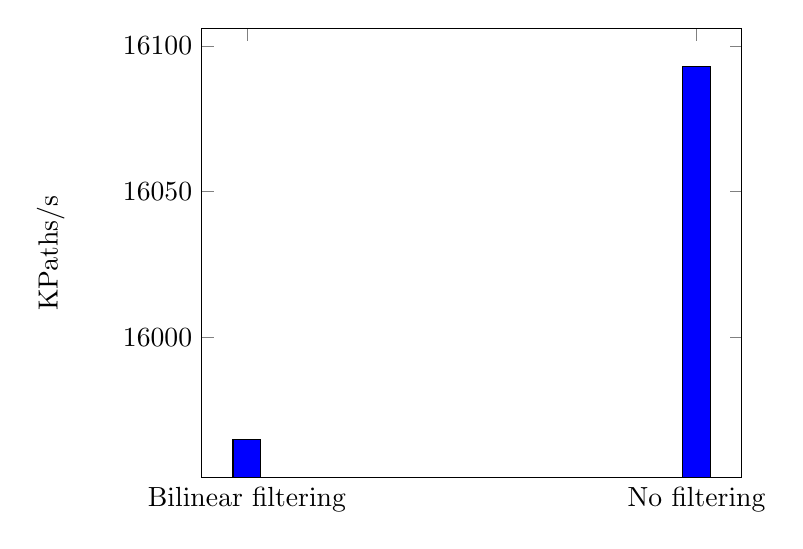
\begin{tikzpicture}
       \begin{axis}[
           symbolic x coords={Bilinear filtering, No filtering},
           xtick=data,
		/pgf/number format/.cd,
		1000 sep={},
		scaled y ticks=false,
		ylabel=KPaths/s,
		ylabel style={yshift=0.5cm},
         ]
           \addplot[ybar,fill=blue] coordinates {
               (Bilinear filtering,   15965)
               (No filtering,  16093)
           };
       \end{axis}
\end{tikzpicture}
\caption{Comparación de eficiencia para filtrado / no filtrado.}
\label{fig:filtercomparaison}
\end{figure}
	
\subsection{Mapas de normales}
		
A nivel artístico resulta muy útil definir la normal para cada intersección en un triángulo de manera arbitraria, aporta control sobre la dirección en la que la luz incide en la superficie; además de que permite dar mayor complejidad y detalle a las geometrías contar con la penalización que implica hacer uso de triángulos adicionales. Un ejemplo de esto es la \autoref{fig:normalmap}, donde se puede ver como una simple textura puede simular relieve en la superficie de una esfera a partir de la textura en la \autoref{fig:normalmaptexture}. 
	
		
\begin{figure}[H]
    \centering
	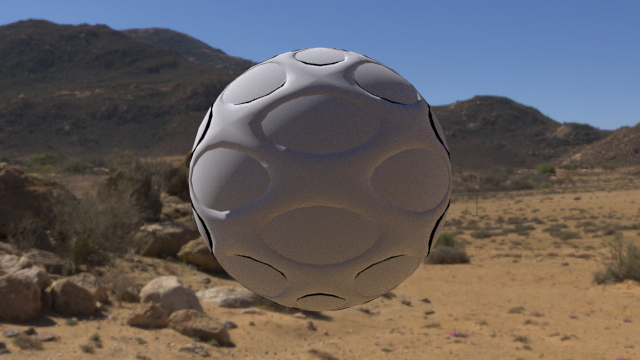
\includegraphics[width=0.6\textwidth]{normalmap}
	\caption{Esfera con mapa de normales.}
	\label{fig:normalmap}
\end{figure}

\begin{figure}[H]
    \centering
	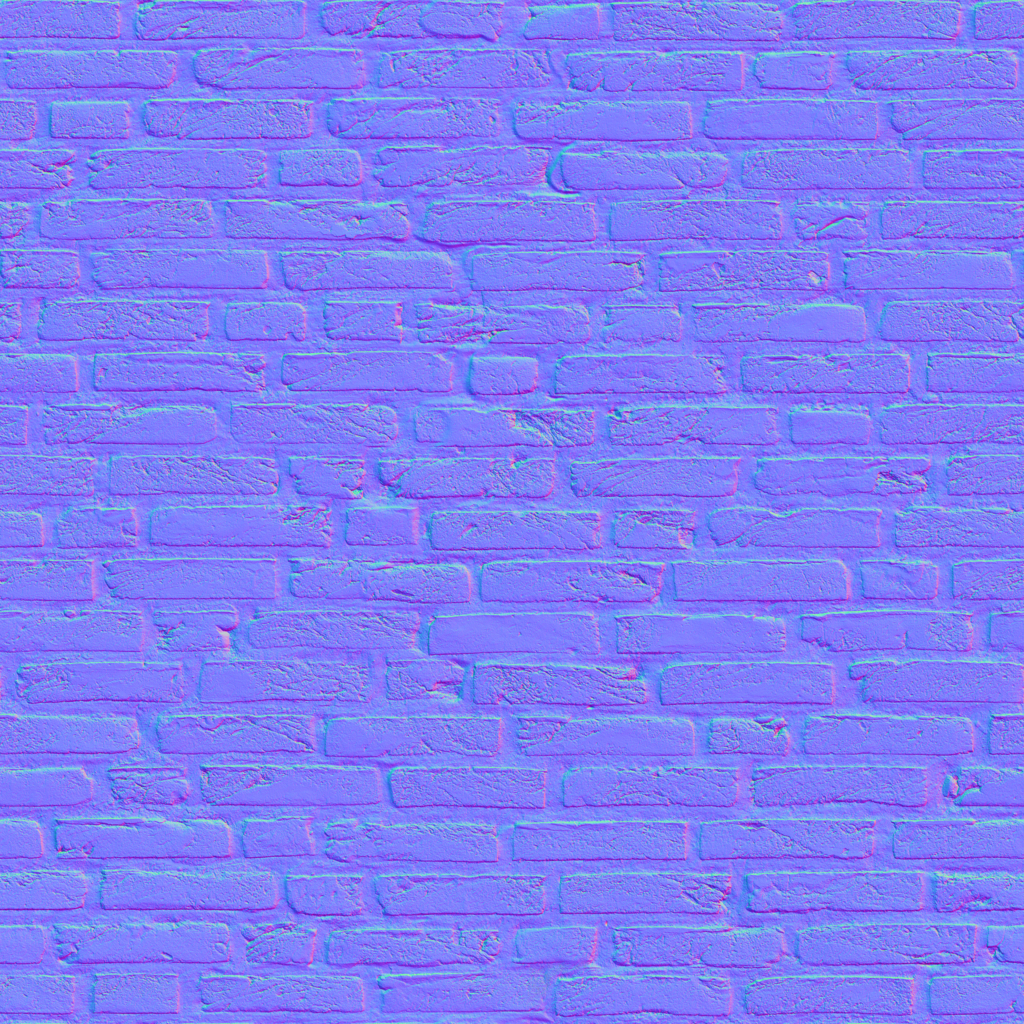
\includegraphics[width=0.3\textwidth]{normalmaptexture}
	\caption{Textura para mapa de normales.}
	\label{fig:normalmaptexture}
\end{figure}


	
La mayor parte de la información acerca de los mapas de normales se ha obtenido en LearnOpenGL.com \cite{learnopengl}, donde se explican las nociones teóricas sobre estos.
	
Estas normales se suministran a través de texturas de una forma similar a la mencionada anteriormente. La textura que carga la información del mapa de normales cuenta con tres canales de color. Cada canal se utiliza para definir la coordenada de la normal, siendo el canal rojo la coordenada \code{x}, el canal azul la coordenada \code{y} y el canal verde la coordenada \code{z}.

La conversión de un color a una normal se hace con el siguiente código: \code{localNormal = (color * 2) - 1;} ya que las coordenadas de la normal se encuentran en el rango [-1, 1] y los valores de color se encuentran en el rango [0,1).
	
Hasta ahora, en ningún momento se ha tenido en cuenta el espacio en el que se encuentran estas normales. Los vectores suministrados por los mapas de normales son locales en el espacio tangencial. El espacio tangencial es un espacio formado por la normal calculada a partir del triángulo, la tangente y la bitangente, tres vectores aproximadamente ortogonales. La representación visual de estos tres vectores que forman el espacio tangencial se muestra en la \autoref{fig:tangentspace}.

\begin{figure}[H]
    \centering
	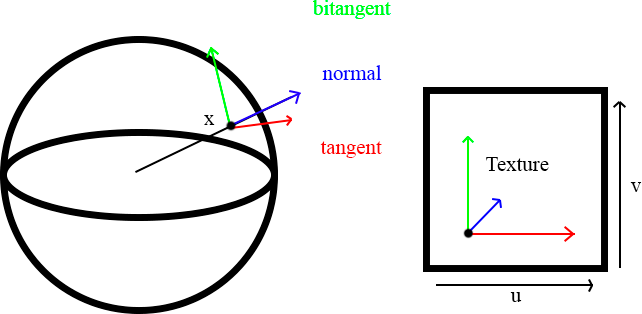
\includegraphics[width=0.4\textwidth]{tangentspace}
	\caption{Espacio tangencial y su proyección en una textura.}
	\label{fig:tangentspace}
\end{figure}
	
Las normales que se han utilizado hasta ahora para los cálculos de iluminación son normales globales (world normals), en la base ortonormal. La conversión de un vector en el espacio tangencial al global se realiza de la siguiente manera: \code{worldNormal = (localNormal.x * tangent - localNormal.y * bitangent + localNormal.z * normal).normalized()}
	
El cálculo de la tangente y bitangente a partir de la normal no es un cálculo trivial, hay infinitos vectores ortogonales que pueden formar esta base. Morten Mikkelsen \cite{mikkelsen2008simulation} propone un método estandarizado para calcular este espacio tangencial y además aporta una implementación en C en su repositorio \cite{mikktspace}. Gran parte de los programas de diseño 3D utilizan este método o uno compatible. Por esa razón se ha decidido hacer uso de él. El método en sí se encarga de cada caso específico, como por ejemplo polígonos degenerados, pero en su esencia calcula la tangente en dirección al incremento de la coordenada \code{u} en el triángulo y la bitagente en dirección de la coordenada \code{v}. Este proceso se explica de manera más detallada en un árticulo de LearnOpenGL \cite{learnopengl}.

Para hacer uso de la implementación MikkTSpace tan solo hay que definir un archivo adicional que enlace las funciones de callback, que solicitarán parámetros para el cálculo de las tangentes tales como las posiciones de los vértices, el número de triángulos etc.

	
\section{Smooth Shading}
	
En \hyperref[subsec:triintersection]{Intersección triángulo - rayo} se explica cómo las normales son calculadas a partir de la superficie que forma el triángulo. Para modelos con poca cantidad de triángulos, este método de cálculo de la normal de la superficie puede resultar insuficiente.
	
Un arreglo sencillo consiste en aplicar el método conocido como Smooth Shading. 
	
Para este método es necesario precalcular una normal por cada vértice, algo que hacen casi todos los programas de diseño 3D. En el caso de los ficheros .obj, estas son definidas con el prefijo "vn". Una vez se cuenta con dichas normales, es necesario interpolarlas. 

Por ello, en la función \code{hit()} de \code{Tri} se añade el código determinado en \autoref{cod:smoothshading}

\begin{minipage}[c]{0.95\textwidth}
\begin{lstlisting}[label={cod:smoothshading}, caption={Código interpolación de normales.}]
			
	#if SMOOTH_SHADING 

    Vector3 shadingNormal  = normals[0] + (normals[1] - normals[0]) * u + (normals[2] - normals[0]) * v;
    Vector3 shadingTangent = tangents[0] + (tangents[1] - tangents[0]) * u + (tangents[2] - tangents[0]) * v;

\end{lstlisting}
\end{minipage}
	
Tanto la normal y la tangente son interpoladas a partir de las coordenadas baricéntricas del triángulo \code{u,v}, las cuales indican la distancia a cada vértice, como se muestra en la \autoref{fig:smoothshading}. El resultado de implementar "Smooth Shading" queda reflejado en las figuras \autoref{fig:smoothshadingoff} y \autoref{fig:smoothshadingon}, donde la primera es un ejemplo de esta característica desactivada y la segunda es un ejemplo de la característica activada.
	
\begin{figure}[H]
    \centering
	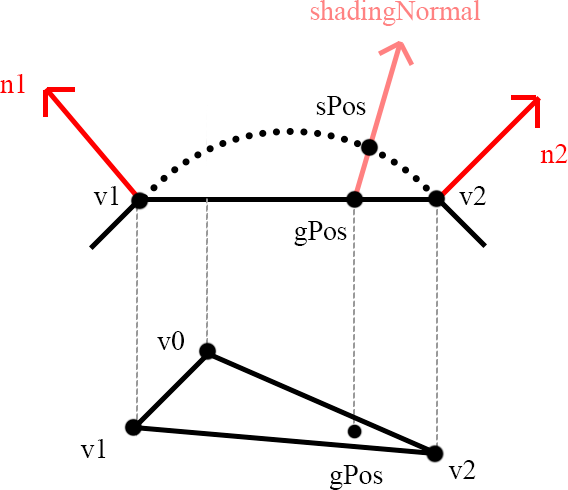
\includegraphics[width=0.3\textwidth]{smoothshading}
	\caption{Interpolación de normales.}
	\label{fig:smoothshading}
\end{figure}

\begin{figure}[H]
		\centering
		\begin{minipage}[b]{0.4\textwidth}
		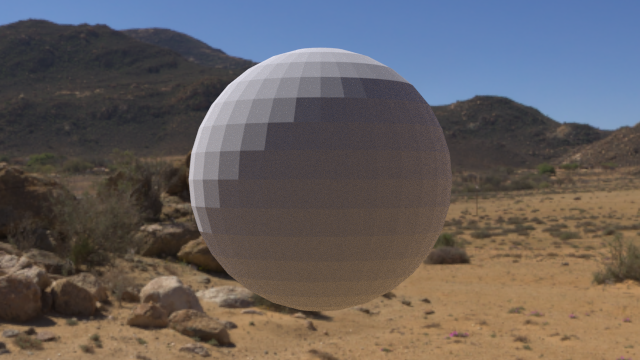
\includegraphics[width=\textwidth]{smoothshadingoff}
		\caption{Smooth Shading desactivado.}
		\label{fig:smoothshadingoff}
	  \end{minipage}
	  \hfill
	  \begin{minipage}[b]{0.4\textwidth}
		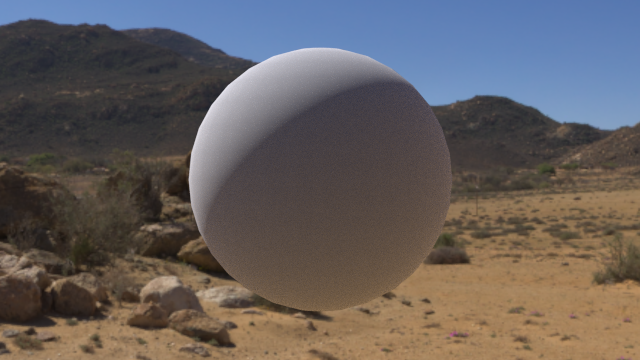
\includegraphics[width=\textwidth]{smoothshadingon}
		\caption{Smooth Shading activado.}
		\label{fig:smoothshadingon}
	  \end{minipage}
	  	\hfill
\end{figure}


Al implementar esta mejora pueden aparecer artefactos conocidos como "Shadow Terminator Arctifact". El uso de una normal interpolada implica que se está haciendo uso de una normal que no coincide con la posición de la superficie. Esta discrepancia crea artefactos visuales presentes hasta en las implementaciones más actualizadas de Blender Cycles, véase por ejemplo la \autoref{fig:shadowterminatorcycles}. Mauricio Vives en \cite{shadowterminatorrepo} propone una solución a este problema y es computar una nueva posición de la superficie a partir de la proyección de la antigua posición al plano que define cada vértice y su normal. Estas tres proyecciones son interpoladas de la misma manera que con las normales, haciendo uso de las coordenadas baricéntricas.
	
\autoref{cod:shadowterminator} muestra el código adaptado a Eleven Renderer.

\begin{minipage}[c]{0.95\textwidth}
\begin{lstlisting}[label={cod:shadowterminator}, caption={Código Shadow Terminator.}]
	
	Vector3 p0 = projectOnPlane(geomPosition, vertices[0], normals[0]);
    Vector3 p1 = projectOnPlane(geomPosition, vertices[1], normals[1]);
    Vector3 p2 = projectOnPlane(geomPosition, vertices[2], normals[2]);

    Vector3 shadingPosition = p0 + (p1 - p0) * u + (p2 - p0) * v;

    bool convex = Vector3::dot(shadingPosition - geomPosition, shadingNormal) > 0.0f;
	
	hit.position = convex ? shadingPosition : geomPosition;
	
\end{lstlisting}
\end{minipage}

El resultado de la implementación en Eleven Renderer se muestra en la \autoref{fig:shadowterminatoreleven}

\begin{figure}[H]
	\centering
	  \begin{subfigure}[b]{0.4\textwidth}
		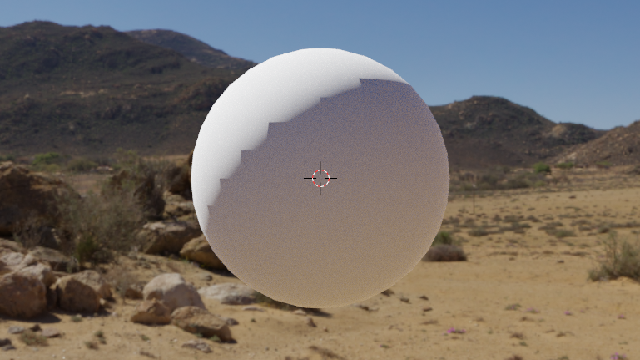
\includegraphics[width=\textwidth]{shadowterminatorcycles}
		\caption{Escena de esfera en Cycles.}
		\label{fig:shadowterminatorcycles}
	  \end{subfigure}
	 \hfill
	  \begin{subfigure}[b]{0.4\textwidth}
		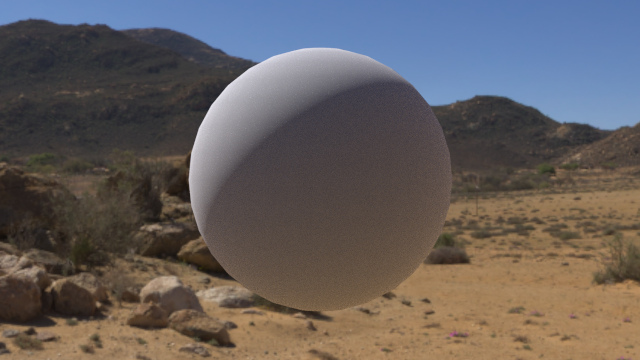
\includegraphics[width=\textwidth]{shadowterminatoreleven}
		\caption{Escena de esfera en Eleven Renderer.}
		\label{fig:shadowterminatoreleven}
	  \end{subfigure}
	  \caption{Artefactos visuales y solución debidos a Shadow Termination.}
      \label{fig:shadowterminator}
	 \hfill
\end{figure}
	
\section{Sombreado BRDF}
	
El sombreado (shading) es el proceso por el cual se asigna un valor de pérdida de energía para un rayo que intersecciona con un punto. Este proceso simula el proceso natural de la interacción entre un haz de fotones y una superficie, dónde parte de los fotones son absorbidos dependiendo de distintos factores como la longitud de onda de los fotones, el tipo de superficie, el tipo de material (los metales reflejarán de manera menos aleatoria que los materiales dieléctricos). La simulación de estas interacciones y simplificación en una función es una ciencia conocida como PBR, o Physically Based Rendering, donde se trata de imitar de manera fiel la realidad física. 
		
En la ecuación de renderizado se encuentra un término denominado BRDF $f_{\text{r}}(\mathbf {x} ,\omega _{\text{i}},\omega _{\text{o}})$. Hasta ahora ha sido ignorado y simplificado como una superficie Lambertiana perfectamente difusa, es decir que se ha tratado la luz independientemente del ángulo de incidencia $\omega _{\text{i}}$ y del ángulo de reflexión del rayo $\omega _{\text{o}}$. En el momento en el que se tienen en consideración estos dos ángulos, se pueden configurar funciones complejas que determinen distintos coeficientes para distintos ángulos. Una función BRDF basada en comportamientos físicos reales como los mencionados anteriormente ofrecerá un resultado acercado a la realidad. 
	
Disney propone una función BRDF conocida como Disney Principled BRDF\cite{burley2012physically}. Este modelo ha sido ideado por Disney con el fin de adaptar los parámetros del modelo de sombreado a unos parámetros amigables para los artistas. Con esto se pretende dejar de lado los antiguos modelos de sombreado poco intuitivos. Esta función de sombreado es utilizada también por Blender Cycles como modelo predeterminado.
	
El término \emph{material} y \emph{BRDF} están fuertemente ligados. Un material es un conjunto de valores para estos atributos.
		
Así pues se procede a explicar estos atributos sintetizados:

\begin{itemize}

	\item Albedo: Color base.
	\item Emission: Energía lumínica añadida, el término $L_{\text{e}}(\mathbf {x} ,\omega _{\text{o}})$ de la ecuación de renderizado.
	\item Roughness: Rugosidad de una superficie.
	\item Metallic: Como de metálica es una superficie, cuanto menor sea la cantidad, más dieléctrico el material.
	\item Clearcoat: Capa de barniz superior.
	\item ClearcoatGloss: Lo pulida que está dicha capa de barniz.
	\item Anisotropic: Distorsión de la luz propia de los metales.
	\item Specular: Cantidad de reflejo especular.
	\item SpecularTint: Color de dicho reflejo.
	\item Sheen: Cantidad de luz en los bordes del material.
	\item SheenTint: Color de la capa de luz anterior.
	\item Subsurface: Sub Surface Scattering falso simulado.
	
\end{itemize}

En Eleven Renderer se ha hecho uso de una implementación ya existente \cite{knightcrawler25} de las ecuaciones del shader de Disney adaptada sin utilizar la transmisión. El propio Disney tiene en Github implementaciones de este shader disponibles \cite{disneyrepo}. Se compara en la \autoref{fig:materialtest} tres parámetros distintos en Eleven Renderer. La primera hilera muestra distintos valores de \emph{albedo}, la segunda muestra la variación de \emph{rougness} incrementando de izquierda a derecha, siendo los materiales de la derecha más lisos. En la tercera hilera se muestra una comparativa del parámetro \emph{metallic}, siendo los materiales de la derecha más metálicos.

Gracias a la implementación previa de texturas es posible además definir estos valores de manera arbitraria para distintas partes del objeto.

\begin{figure}[H]
	\centering
	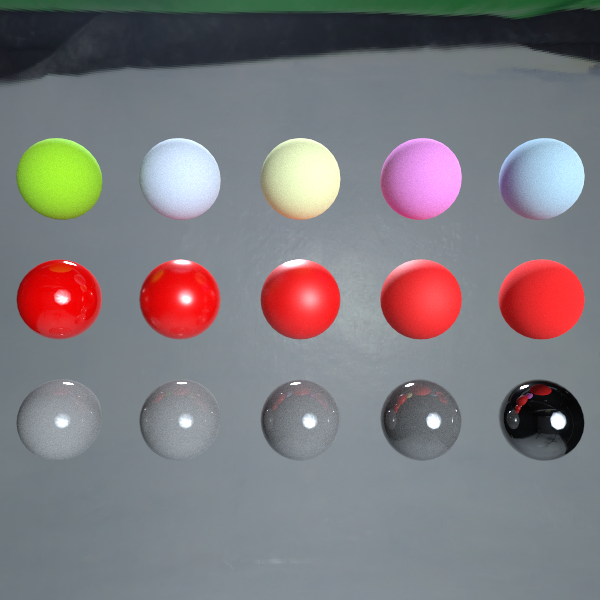
\includegraphics[width=0.5\textwidth]{materialtest}
	\caption{Comparación de los atributos albedo, roughness y metallic.}
	\label{fig:materialtest}
\end{figure}
	
